\chapter{Estado del Arte} \label{chap:estadodelarte}
En el siguiente capítulo se  expondrá las diversas investigaciones realizadas en el ámbito espacial aplicando técnicas de visión artificial para el reconocimiento de patrones. En primer lugar se van a explorar los trabajos que que se realizaron sobre imágenes  satelitales; por ultimo vamos a detallar las investigaciones y trabajos llevados a cabo en vuelo.

\section{Aplicaciones en el ámbito espacial}\label{sec:estadodelacuestion}

Las aplicaciones de visión artificial en el ámbito espacial son cada ves mas utilizadas, esto se debe principalmente a dos factores muy importantes; como primer lugar la creciente capacidad de computo de procesamiento con procesadores de mayor capacidad y el auge de las GPU, unidad de procesamiento gráfico. En segundo lugar la aparición de algoritmos y frameworks mas eficiente para el uso en reconocimiento de patrones; de los que podemos nombrar el uso de \ac{cnn}. Otro tema no menos importante son la aparición de UAVs usados para el reconocimiento de patrones. La presencia en el mercado de pequeños UAVs de bajo costo con capacidad para portar pequeñas cámaras de vídeo de alta resolución y de realizar despegue vertical con posibilidad de 
movimiento en cualquier dirección del espacio, hace posible abordar nuevos retos en el campo de la detección y seguimiento de determinadas situaciones de la realidad \citep{Lanillos}.

Actualmente en el campo de reconocimiento de patrones la mayoría de los trabajos que se realizaron en el área espacial han sido aplicado en tierra utilizando para estos imágenes satelitales en los diversos estudios sobre las característica del terreno. Estas aplicaciones son cada vez mas explotada no solo por agencias espaciales sino en entidades educativas, publicas o privadas. 

Como se mencionó previamente esta sección se dividirá en dos partes; por un lado los trabajos realizados en tierra, de mayor uso, y por otro las investigaciones y trabajos realizados en vuelo.

Para empezar vamos a comenzar citando el siguiente trabajo realizado por \citep{Cheang}; en este articulo se describe el uso de técnicas de reconocimiento de patrones usando aprendizaje supervisado. El método para la extracción y clasificación de los datos utilizado se baso en dos enfoques; por una parte utilizaron técnicas de \textit{sliding window} para la obtención de regiones candidatas, por otro se aplicaron redes neuronales profundas, \ac{dl}, método muy utilizado en estos trabajos, para el reconocimiento del objeto. Otro ejemplo encontrado en la literatura aplicando  \textit{aprendizaje no supervisado} para la clasificación del uso de la tierra a partir de imágenes satelitales multi-temporales, en este paper \citep{pnn}, se utilizo imágenes del satélite LANSAT y SPOT usando redes neuronales probabilística, estas técnicas realizan un agrupamiento de datos, \textit{clusters}, y realizan la clasificación creando las fronteras entre los diferentes \textit{clusters} de datos para su posterior reconocimiento.

La \ac{va} permite crear mapas urbanos a partir de imágenes satelitales como se menciona en el articulo \citep{detectionHOG}. Aplicando \ac{va} se crearon mapas urbanos para determinar los cambios temporales que ocurrieron en una región. En este trabajo los autores proponen dos módulos para el desarrollo, por un lado usar \textit{HOG} \footnote{Fuente:\url{https://en.wikipedia.org/wiki/Histogram_of_oriented_gradients}} para la extracción de características en la imagen y \textit{Local binary patterns (LBP)}\footnote{Fuente:\url{https://en.wikipedia.org/wiki/Local_binary_patterns}}, como método descriptor de característica; por ultimo para la calificación utilizando técnicas SVM (ver:\ref{sub:svm}). \cite{usman} en su articulo describe la extracción de características de una imagen satelital aplicando métodos de  detección de bordes, \textit{edges proposal}, para el 
reconocimiento de límites catastrales.

Como se vio en lo expuesto anteriormente, son diversos los trabajos e investigaciones que se realizaron utilizando algoritmos de reconocimiento de patrones sobre imágenes satelitales. En aplicaciones de vuelo son mucho menor los ejemplo encontrados en la literatura, esto se debe a la escasez de recursos computacionales en vuelo; en los recientes años esta problemática esta mutando debido al avance del poder de computo con herramientas tecnológicas de gran capacidad de procesamiento como son las \textit{GPU (Unidad de procesamiento gráfico)}, esto nos da un nuevo enfoque a la hora de pensar en realizar procesamiento en vuelo.

Unos de los ejemplos destacados de aplicación de técnicas de \ac{va} en vuelo, no podemos dejar de mencionar al \textit{Dr.Tweddle} que en su trabajo, \textit{Computer Vision Based Navigation for Spacecraft Proximity Operations}, estudia y detalla el uso de \ac{va} para realizar una navegación autónoma en satélites; en esta tesis destaca el proyecto de un Nanosatélite, CubeSat, de la \ac{nasa} llamado , Synchronize Position Hold Engage and Reorient Experimental Satellite (\textit{SPHERES}), que dispone de un modo experimental del uso de tecnología de visión artificial, señalando la ventaja del uso de esta tecnología en relación a otra tecnología de sensado \citep{Brent}.

En el espacio ya existen aplicaciones desarrolladas que utilizan algoritmos de \ac{va}. Las aplicaciones que utilizan estas técnicas mayormente están orientada en el aprendizaje autónomo. Debido a las grandes distancias que existen, es necesario lograr cierta autonomía en la toma de decisiones ya que comandar desde tierra es inviable debido al retardo de la comunicación; es el ejemplo del \textit{Mars Rover}, robot desarrollado para la exploración de la superficie de Marte crea mapas de entorno para saber donde se encuentra y así poder detectar diversos obstáculos \citep{RoverMars}. 
El uso de \ac{va} tiene un rol importante en el incremento de autonomía; usando \ac{va} para el reconocimiento de patrones permite realizar manipulaciones de objetos brindando soporte a astronautas en el espacio. En la investigación realizada por la \ac{nasa} se destaca el reconocimiento de patrones utilizando un robot por medio de diferentes cámaras que captan la profundidad y posición del objeto para poder realizar un reconocimiento óptimo \footnote{Fuente: 
http://blog.infaimon.com/robots-guiados-por-vision-artificial-para-el-espacio-robos-guiados-por-visao-artificial-para-o-espaco/}.

El proyecto \textit{Docking and Capture of Satellites through computer vision}, ASIROV: Acoplamiento y Agarre de Satélites mediante Sistemas Robóticos basado en Visión \footnote{Fuente: https://goo.gl/w7iayv}, desarrollado para atracar y capturar satélites espaciales se basa  en tecnologías de \ac{va} para guiar de forma autónoma un vehículo espacial.

Usar técnicas de \ac{va} implica lograr que el satélite tenga mayor autonomía, en el articulo realizado por \cite{Kouyama}, aplica reconocimiento de patrones para determinar la actitud y órbita del satélite basado en los datos adquiridos por los sensores del mismo. En el articulo los autores describen que para pequeños satélites,CubeSat, tienen una carga útil limitada y sus actitudes a veces son difíciles de determinar a partir de los pocos sensores que contiene a bordo por sí solos. Estas actitudes incorrectas conducen a proyecciones y mediciones inexactas que requieren corrección de pos-procesamiento en tierra. En el estudio proponen un esquema automatizado y robusto que deriva la actitud del satélite a partir de sus imágenes de observación y de la posición de satélite conocida, combinando características de tierra de una imagen observada y de imágenes registradas. El esquema combina algoritmos de \ac{va} (es decir, detección de características y validaciones robustas) y restricciones geométricas de la observación por satélite. \cite{Huggins} en su trabajo titulado \textit{Computer Vision Localization Based on Pseudo-Satellites} propone usar técnicas de \ac{va} para la localización y orientación de un CubeSat para complementar la navegación. El estudio se enfoca en  aumentar la capacidad de los GPS utilizando \ac{va}. Este trabajo  siguiere crear una red de nodos en el cual un grupo de nodos poseen GPS para calcular su posición y el otro grupo a partir del uso de la posición de la cámara y usando técnicas de  \ac{va}  utilizar la posición del primer grupo para calcular la suya intercambiando información de los datos y calculando la distancia y orientación de la cámara \citep{Huggins}.

Como vimos existen en la actualidad estudios y aplicaciones realizadas ya sea en vuelo o en tierra que utilizan algoritmos de reconocimiento de patrones, por lo que la tendencia vista en los últimos tiempo es muy alentadora y nos abre una nueva forma de mirar al espacio y enfocar nuestro desarrollo a esta área, como podemos ver en el gráfico siguiente \ref{Fig: scopus1}. Los datos que muestran el \ref{Fig: scopus2} han sido relevados desde el año 2000 hasta la fecha.

\begin{figure}[h]
 \centering
  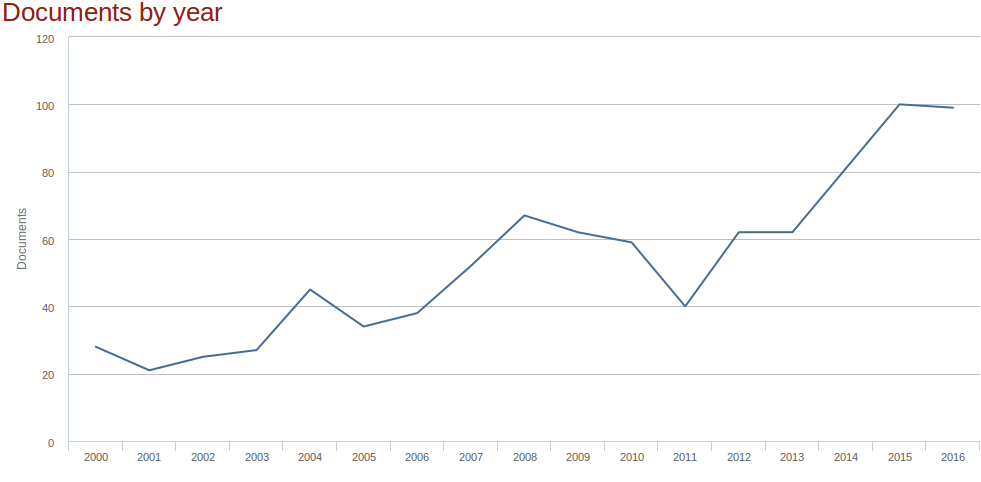
\includegraphics[height=7cm,keepaspectratio=true,clip=true]{imagenes/Logos/scopus.png}
  \caption{Extraído de Scopus.com}
	\label{Fig: scopus1}
\end{figure}

\begin{figure}[h]
 \centering
  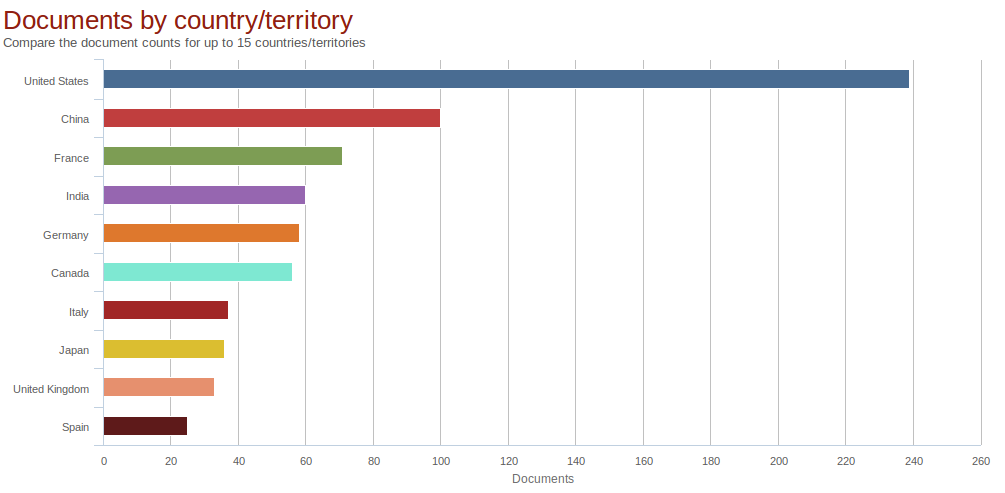
\includegraphics[height=7cm,keepaspectratio=true,clip=true]{imagenes/Logos/scopus2.png}
  \caption{Extraído de Scopus.com}
	\label{Fig: scopus2}
\end{figure}


